\documentclass[conference]{IEEEtran}
\IEEEoverridecommandlockouts
\usepackage{cite}
\usepackage{amsmath}
\usepackage{graphicx}
\usepackage{booktabs}
\usepackage{multirow}
\usepackage{xcolor}
\usepackage{url}
\usepackage{textcomp}
\usepackage{float}
\def\BibTeX{{\rm B\kern-.05em{\sc i\kern-.025em b}\kern-.08em
    T\kern-.1667em\lower.7ex\hbox{E}\kern-.125em X}}

\begin{document}

\title{Are AI Agents Treated Like Teammates? An Empirical Study of Pull Request Outcomes on GitHub}

\author{\IEEEauthorblockN{Saman Shaheen}
\IEEEauthorblockA{\textit{Polytechnique Montr\'eal}\\
Montr\'eal, Canada\\
saman.shaheen@etud.polymtl.ca}
\and
\IEEEauthorblockN{[\'Emilie Larocque]}
\IEEEauthorblockA{\textit{Polytechnique Montr\'eal}\\
Montr\'eal, Canada\\
\relax[emilie.larocque@etud.polymtl.ca]}
\and
\IEEEauthorblockN{[Eugenia Carcea]}
\IEEEauthorblockA{\textit{Polytechnique Montr\'eal}\\
Montr\'eal, Canada\\
\relax[eugenia.carcea@etud.polymtl.ca]}
\and
\IEEEauthorblockN{[Randy M\'egane Rakotondrazafy]}
\IEEEauthorblockA{\textit{Polytechnique Montr\'eal}\\
Montr\'eal, Canada\\
\relax[randy-megane.rakotondrazafy@etud.polymtl.ca]}
}

\maketitle

\begin{abstract} 
Autonomous coding agents can now generate and submit pull requests (PRs) on GitHub, creating a new form of human--AI collaboration in software development. However, little is known about how maintainers interact with these contributions compared with human-authored PRs. This study analyzes 21,740 PRs from the AIDev dataset and compares development outcomes and collaboration patterns between AI-agent and human contributions. AI-generated PRs are merged less often than human PRs (72.9\% vs.\ 80.8\%), but accepted PRs are merged substantially faster. They also receive much less review and discussion activity. In particular, only 13.5\% of AI PRs receive an approving review compared with 47.5\% of human PRs. Overall, the results suggest that AI-generated contributions are often treated as delegated output rather than collaborative work requiring extensive discussion and review. 
\end{abstract}

\begin{IEEEkeywords}
AI teammates, pull requests, mining software repositories, human--AI collaboration, code review
\end{IEEEkeywords}

\section{Introduction}
Autonomous coding agents such as OpenAI Codex, Devin, GitHub Copilot, Cursor, and Claude Code are increasingly capable of producing software changes and submitting them as pull requests (PRs) \cite{li2025rise}. As these systems become part of the software development process, they create a new form of human--AI collaboration in which developers review, discuss, and integrate AI-generated contributions. Pull requests provide a detailed record of software collaboration. They capture development outcomes such as merge decisions and review activity, as well as collaboration behaviors including comments, feedback, and discussion patterns. Mining software repositories therefore provides an opportunity to study how AI-generated contributions are treated in practice. This report compares AI-agent and human pull requests along two dimensions proposed in the course project: development outcomes and collaboration patterns. Understanding these differences can help researchers and practitioners better understand the role that autonomous coding agents currently play in software engineering workflows.

\section{Research Questions} 
Two research questions guide our analysis of AI-agent and human pull requests: \\
\textbf{RQ1 (Development Outcomes).} How do AI-agent pull requests differ from human pull requests in terms of merge rate, closing rate, time to merge, and review activity? \\
\textbf{RQ2 (Collaboration Patterns).} How do collaboration practices differ between AI-agent and human pull requests in terms of discussion volume, reviewer participation, conversational exchanges, and review language such as clarification, approval, and rejection?

\section{Methodology}
\subsection{Data collection}
We use the AIDev dataset released with~\cite{li2025rise} (Hugging Face \texttt{hao-li/AIDev}, revision v3), the dataset behind the course repository \texttt{SAILResearch/AI\_Teammates\_in\_SE3}. It lists PRs opened by AI coding agents and, as a baseline, human PRs. We concatenated both tables, removed duplicate PR ids, kept all human PRs, and drew a random 50\% sample of the (much larger) AI table (seed 42). Each PR URL was parsed into owner/repository/number, and every PR was queried through the GitHub GraphQL API~\cite{githubgql} (15 PRs per request) for state, creation/close/merge timestamps, author login and account type, issue comments (first 100), reviews (first 50: state, submission time, body, author) and inline review comments (first 50 per review). The script waits for the rate-limit reset and retries failed batches. Of 23{,}416 sampled PRs, 22{,}710 were retrieved. 706 (3.0\%) no longer resolve (deleted or renamed repositories, disabled PRs) and were dropped. Mining ran in late September 2026.

\emph{Replication package:} \url{https://github.com/Eugenia3/Replication_Project_LOG6307E} (Colab pipeline, data archive, and this report).

\subsection{Cleaning and classification}
\textbf{AI vs.\ human.} We rely on AIDev's group label (PR opened by one of the dataset's AI agents vs.\ a human-authored PR) rather than our own heuristic. \\
\textbf{Bots.} Comments and reviews written by bots (login ending in \texttt{[bot]}, GraphQL type \texttt{Bot}, deleted accounts, or a list of common CI/dependency-bot names) are removed from every PR. Bot-authored \emph{PRs} are discarded only from the human group (970 PRs, 15.1\% of 6{,}423), because agents themselves often post from bot-flagged accounts and discarding them would empty the AI group. The final dataset contains 21{,}740 PRs (including 16{,}287 AI, 5{,}453 human). \\
\textbf{Missing values.} PRs without any timestamped comment have no response time (excluded from that test only). The time to merge exists only for merged PRs and counts default to 0. \\
\textbf{Text.} Before counting words and matching keywords, comment bodies are stripped of HTML comments, code blocks, inline code, images, quoted lines, HTML tags and URLs. \\
\textbf{Language classes.} Three hand-written regular-expression lexicons flag explanation requests (e.g., ``is this intentional'', ``could you elaborate and explain''), approval (``LGTM'', ``looks good'', ``approved'') and rejection (``please fix/revert'', ``do not merge'', ``incorrect'') in any comment or review. Task-type classification was not needed for RQ1/RQ2.

\subsection{Metrics}
Table~\ref{tab:metrics} defines the per-PR metrics. All of them are computed after cleaning.

\begin{table}[H]
\caption{Metric definitions (one value per PR).}
\label{tab:metrics}
\centering\small
\begin{tabular}{@{}p{0.95in}p{2.4in}@{}}
\toprule
Metric & Definition \\
\midrule
Merge / close rate & Share of PRs with a merge / close timestamp (closed includes merged) \\
Time to merge & mergedAt $-$ createdAt, hours (merged PRs only) \\
Reviews & Number of non-bot reviews \\
Comments & Issue comments + reviews + inline review comments (non-bot) \\
Reviewers / participants & Distinct review authors / distinct authors of any comment or review \\
Comment length & Mean words per non-empty cleaned comment \\
First response$^\dagger$ & Earliest timestamped comment $-$ createdAt, hours \\
Alternations$^\dagger$ & Switches between PR author and others in the chronological comment sequence \\
Language flags & $\geq$1 clarification / approval / rejection match in the PR \\
Review outcome & $\geq$1 review in state APPROVED / CHANGE\_REQUESTED\\
\bottomrule
\end{tabular}
\\[2pt]\footnotesize $^\dagger$ See Threats to Validity:  The data lacks time stamps and is affected by bot-filtering issues. 
\end{table}

\subsection{Analysis}
Binary metrics are compared with $\chi^2$ tests of independence (SciPy default, Yates correction for $2{\times}2$ tables) and numeric metrics with two-sided Mann--Whitney U tests~\cite{mannwhitney}, because the distributions are skewed and zero-inflated. With $N\approx 21{,}700$ almost any difference is significant, so we also report effect sizes computed from the test outputs: the odds ratio (OR) for binary metrics and the probability of superiority $P(\mathrm{AI}{>}\mathrm{H})=U/(n_{AI}n_{H})$ for numeric ones (0.5 means no difference). We run 15 tests and use a Bonferroni-adjusted $\alpha=0.05/15\approx0.0033$. Analysis uses SciPy~\cite{scipy} and matplotlib.

\section{Results}
Table~\ref{tab:results} summarises all tests, while Figs.~\ref{fig:rq1} and~\ref{fig:rq2} visualise the main contrasts.

\textbf{RQ1 -- Observations.} 
AI PRs are merged less frequently than human PRs (72.9\% vs.\ 80.8\%, OR 0.64), although the effect is relatively small ($\varphi \approx 0.08$). Closing rates are nearly identical (98.1\% vs.\ 98.4\%), indicating that most pull requests eventually reach a resolution regardless of authorship. The main difference lies in the outcome: AI PRs are more likely to be closed without being merged. Among merged pull requests, AI contributions are integrated much faster, with a median merge time of 0.046 hours (approximately 2.7 minutes) compared with 4.55 hours for human PRs. AI PRs also receive fewer reviews, with a median of zero reviews compared with one review for human PRs.

\textbf{RQ2 -- Observations.} 
Human interaction with AI PRs is consistently lower across all collaboration metrics. The median AI PR receives no comments, reviewers, or participants, whereas the median human PR receives at least one of each (Fig.~\ref{fig:rq2}, left). The strongest difference appears in review approval: only 13.5\% of AI PRs receive an approving review compared with 47.5\% of human PRs (OR 0.17, $\varphi \approx 0.36$). Clarification language and approval language are approximately four times less common in AI PRs (1.7\% vs.\ 7.1\% and 3.9\% vs.\ 14.5\%, respectively). Rejection language and change requests are also less frequent, although the differences are smaller. Comment length and alternation counts have a median of zero in both groups, indicating that most pull requests receive little discussion. The significant differences for these metrics therefore reflect the greater likelihood of any discussion taking place in human PRs rather than differences in discussion length.

\clearpage
\onecolumn

\begin{table}[t]
\caption{AI-agent vs.\ human PRs. Rates are percentages of PRs. Numeric metrics show medians. $n_{AI}{=}16{,}287$, $n_H{=}5{,}453$, except time to merge (11{,}873 / 4{,}405) and first response (3{,}232 / 2{,}312). Several $p$-values underflowed to 0 in floating point and are shown as $<$0.001. Effect: OR (rates) or $P(\mathrm{AI}{>}\mathrm{H})$ (numeric). $^\dagger$ Interpret with caution (see Threats).}
\label{tab:results}
\centering\small
\begin{tabular}{@{}llrrrrr@{}}
\toprule
 & Metric & AI & Human & Statistic & $p$ & Effect \\
\midrule
\multirow{4}{*}{RQ1} & Merged (\%) & 72.9 & 80.8 & $\chi^2=134.5$ & $<$0.001 & OR 0.64 \\
 & Closed (\%) & 98.1 & 98.4 & $\chi^2=2.59$ & 0.107 & OR 0.82 \\
 & Time to merge (h) & 0.046 & 4.55 & $U=1.21{\times}10^{7}$ & $<$0.001 & 0.23 \\
 & Reviews per PR & 0 & 1 & $U=2.89{\times}10^{7}$ & $<$0.001 & 0.33 \\
\midrule
\multirow{11}{*}{RQ2} & Comments per PR & 0 & 1 & $U=2.70{\times}10^{7}$ & $<$0.001 & 0.30 \\
 & Reviewers per PR & 0 & 1 & $U=2.83{\times}10^{7}$ & $<$0.001 & 0.32 \\
 & Participants per PR & 0 & 1 & $U=2.56{\times}10^{7}$ & $<$0.001 & 0.29 \\
 & Mean words per comment & 0 & 0 & $U=3.22{\times}10^{7}$ & $<$0.001 & 0.36 \\
 & First response (h)$^\dagger$ & 1.08 & 2.10 & $U=3.74{\times}10^{6}$ & 0.973 & 0.50 \\
 & Alternations$^\dagger$ & 0 & 0 & $U=3.41{\times}10^{7}$ & $<$0.001 & 0.38 \\
 & Clarification language (\%) & 1.7 & 7.1 & $\chi^2=389.6$ & $<$0.001 & OR 0.23 \\
 & Approval language (\%) & 3.9 & 14.5 & $\chi^2=753.7$ & $<$0.001 & OR 0.24 \\
 & Rejection language (\%) & 2.4 & 4.1 & $\chi^2=41.3$ & $<$0.001 & OR 0.58 \\
 & Approved review (\%) & 13.5 & 47.5 & $\chi^2=2740.0$ & $<$0.001 & OR 0.17 \\
 & Changes requested (\%) & 2.8 & 4.1 & $\chi^2=22.5$ & $<$0.001 & OR 0.67 \\
\bottomrule
\end{tabular}
\end{table}

\begin{figure}[t]
\centering
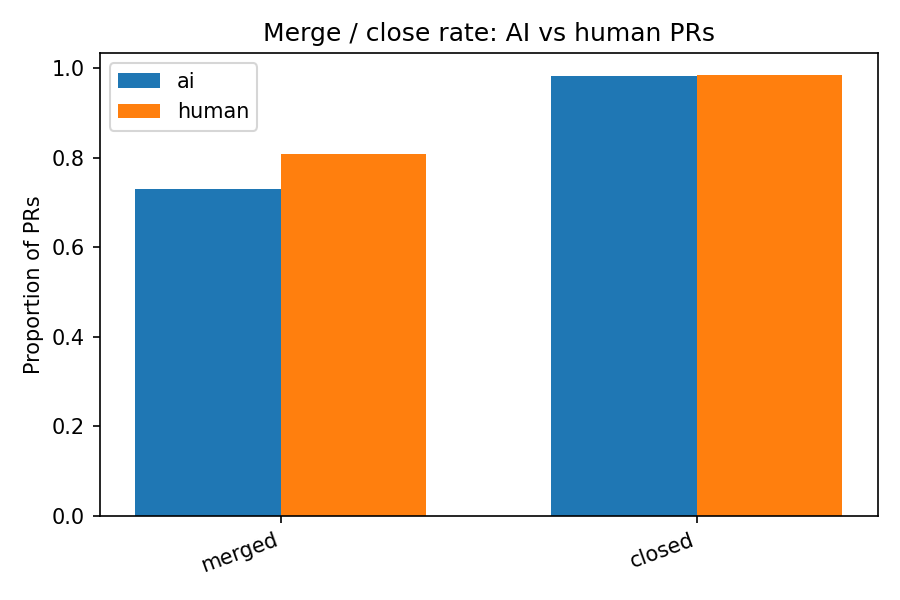
\includegraphics[height=2.2in]{figures/rq1_merge_close_rate_bar.png}\hfill
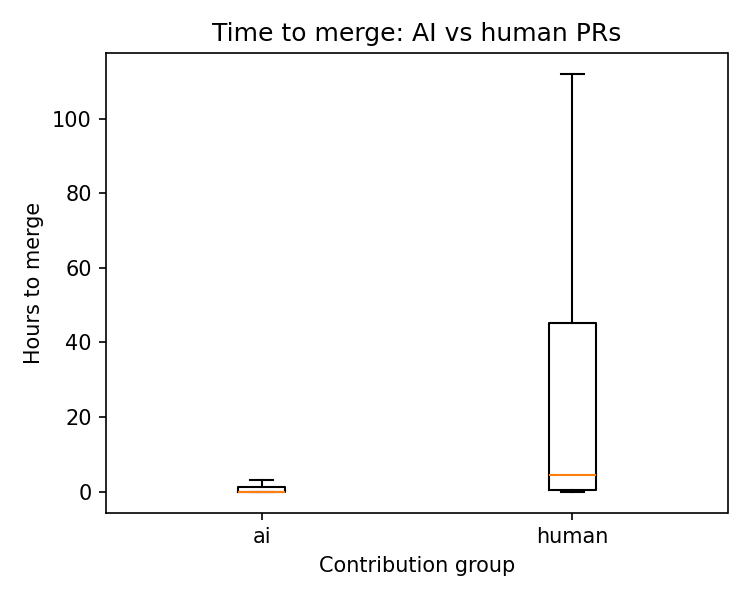
\includegraphics[height=2.2in]{figures/rq1_time_to_merge_boxplot.png}
\caption{RQ1. Left: merge and close rate of AI vs.\ human PRs. Right: time to merge of merged PRs in hours (outliers hidden).}
\label{fig:rq1}
\end{figure}

\begin{figure}[t]
\centering
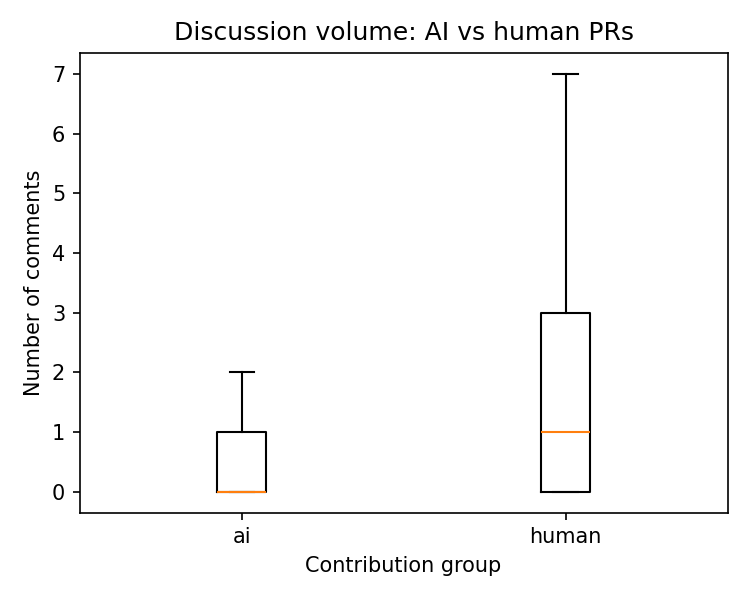
\includegraphics[height=2.2in]{figures/rq2_n_comments_boxplot.png}\hfill
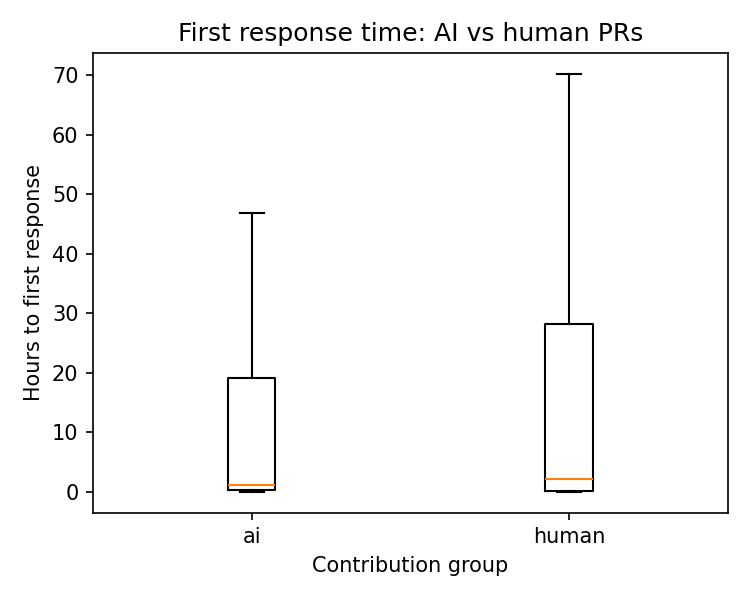
\includegraphics[height=2.2in]{figures/rq2_response_time_boxplot.png}
\caption{RQ2. Left: discussion volume (comments and reviews per PR, outliers hidden). Right: first response time of PRs in hours (outliers hidden).}
\label{fig:rq2}
\end{figure}

\twocolumn

\section{Discussion} 
\textbf{Interpretation.} Taken together, the results suggest that AI-generated pull requests are treated differently from human contributions. AI PRs are merged less frequently, receive considerably less discussion, and often move through the review process with little visible interaction. At the same time, accepted AI PRs are merged much faster than human PRs. One possible explanation is that maintainers view these contributions as delegated output that has already been evaluated before submission. AI-generated changes that meet expectations may therefore be merged quickly, while others are simply closed without extensive discussion. Because merger identity was not mined, this explanation remains a hypothesis. 
\textbf{Human--AI collaboration.} Collaboration around AI PRs appears to be more limited than around human contributions. Clarification requests, approval language, and approval reviews are all substantially less common, suggesting fewer visible review conversations. The largest gap occurs for approving reviews (OR 0.17), indicating that AI-generated contributions frequently move through the development process without the same level of explicit reviewer feedback observed in human PRs. Because agent-authored comments are removed during bot filtering, the analysis primarily captures the human side of the interaction rather than the complete human--AI exchange. 
\textbf{Implications.} As coding agents become increasingly integrated into software development workflows, teams may benefit from establishing explicit review policies for AI-generated contributions. Tool builders may also improve collaboration by making agent reasoning more visible and easier for reviewers to question. More transparent explanations could encourage the clarification and feedback exchanges that currently appear rare in AI-generated pull requests.

\section{Threats to Validity}
\textbf{Timestamps and bots (internal).} Our GraphQL query requested \texttt{submittedAt} for reviews but the metric code reads \texttt{createdAt}. The reviews are therefore ignored by first-response time and ordered incorrectly in the alternation count, and the AI PR author's own replies are typically removed as bot activity, so alternations are biased downward for AI PRs by construction. We mark both metrics ($^\dagger$) and draw no conclusion from them. \\
\textbf{Incomplete metadata.} Comment and review lists are capped (100/50/50), 3.0\% of sampled PRs could not be retrieved, and merger identity, labels, PR size and file changes were not mined. \\
\textbf{AI identification.} We trust AIDev's labels. Human PRs may include unlabeled AI assistance, and the five agents are pooled. \\
\textbf{Classification errors.} Keyword lexicons miss negation, sarcasm and non-English text, and were not validated against manual labels. \\
\textbf{Dataset and repository specificity.} We analyse a 50\% sample of AI PRs and many PRs come from the same repositories, violating test independence and making $p$-values optimistic. The results may not generalise beyond AIDev's repositories or period. \\
\textbf{Missing private context.} Discussions in chat, issue trackers, IDEs or pair sessions are invisible. \\
\textbf{Statistical.} Large $N$ makes tiny differences significant, hence our focus on effect sizes. \\

\section{Conclusion and Future Work} 
This study analyzed 21,740 pull requests from the AIDev dataset to compare development outcomes and collaboration patterns between AI-agent and human contributions. AI-generated pull requests are merged less frequently than human pull requests but are merged substantially faster when accepted. They also receive considerably less human review and discussion. The largest difference was observed for approving reviews, which were almost four times less common for AI-generated contributions. Overall, the results suggest that AI-generated pull requests are often treated as delegated output rather than collaborative contributions that require extensive review and discussion.

\section*{AI-Use Disclosure}
Claude was used to correct grammatical mistakes and format this LaTeX report and to compute effect sizes from the printed test statistics. Data collection, cleaning and statistical analysis were run by the authors in the notebook. The authors reviewed and verified all results and interpretations.

\begin{thebibliography}{99}
\bibitem{li2025rise} H.~Li, H.~Zhang, and A.~E.~Hassan, ``The rise of AI teammates in software engineering (SE) 3.0: How autonomous coding agents are reshaping software engineering,'' arXiv:2507.15003, 2025. Dataset: \url{https://huggingface.co/datasets/hao-li/AIDev}.
\bibitem{githubgql} GitHub, ``GitHub GraphQL API documentation,'' \url{https://docs.github.com/en/graphql}.
\bibitem{mannwhitney} H.~B.~Mann and D.~R.~Whitney, ``On a test of whether one of two random variables is stochastically larger than the other,'' \emph{Ann.\ Math.\ Statist.}, vol.~18, no.~1, pp.~50--60, 1947.
\bibitem{scipy} P.~Virtanen \emph{et al.}, ``SciPy 1.0: Fundamental algorithms for scientific computing in Python,'' \emph{Nature Methods}, vol.~17, pp.~261--272, 2020.
\bibitem{gousios2014pull}
G. Gousios and A. Zaidman, ``A dataset for pull-based development research,'' in \emph{Proc. 11th Working Conf. Mining Software Repositories (MSR)}, 2014, pp. 368--371, doi: 10.1145/2597073.2597122.
\bibitem{kalliamvakou2016github}
E. Kalliamvakou, G. Gousios, K. Blincoe, L. Singer, D. M. German, and D. Damian, ``An in-depth study of the promises and perils of mining GitHub,'' \emph{Empirical Software Engineering}, vol. 21, no. 5, pp. 2035--2071, 2016, doi: 10.1007/s10664-015-9393-5.
\bibitem{rigby2015review}
P. C. Rigby, A. Bacchelli, G. Gousios, and M. Mukadam, ``A mixed methods approach to mining code review data: Examples and a study of multi-commit reviews and pull requests,'' in \emph{The Art and Science of Analyzing Software Data}. Morgan Kaufmann, 2015, pp. 231--255.
\bibitem{copilot2022pair}
S. Imai, ``Is GitHub Copilot a substitute for human pair-programming? An empirical study,'' in \emph{Proc. IEEE/ACM 44th Int. Conf. Software Engineering: Companion Proc. (ICSE-Companion)}, 2022, pp. 319--321, doi: 10.1109/ICSE-Companion55297.2022.9793778.
\bibitem{li2026aidev}
H. Li, H. Zhang, and A. E. Hassan, ``AIDev: Studying AI coding agents on GitHub,'' arXiv:2602.09185, 2026. [Online]. Available: \url{https://arxiv.org/abs/2602.09185}
\bibitem{goldkrinke2022ethics}
N. E. Gold and J. Krinke, ``Ethics in the mining of software repositories,'' \emph{Empirical Software Engineering}, vol. 27, art. no. 17, 2022, doi: 10.1007/s10664-021-10057-7.
\bibitem{mazloomzadeh2026}
I. Mazloomzadeh, M. M. Morovati, and F. Khomh, ``How do AI coding agents contribute to software development? An empirical study of agentic pull requests,'' arXiv:2607.21832, 2026. [Online]. Available: \url{https://arxiv.org/abs/2607.21832}
\end{thebibliography}

\end{document}